\addchapheadtotoc
\chapter{Solver Performance}\label{chapter:Example}
The complexity of the radiation solver resulting from both its theoretical foundation as well as its computational implementation calls for an extensive series of validation and performance studies.
Three test geometries are presented in this chapter for verification and profiling using the two methods discussed in section \ref{section:ModelForThisStudy}. The new MCRT models using the bounding volume hierarchy approach will be refered to as MCRT-ArborX, and the model without will be referred to as MCRT-Standard. 
A well-established Fortran implementation developed over the course of many years will be used for comparison, and will be refered to as MCRT-Fort.
The configurations include the canonical one-dimensional plane-parallel medium, a three-dimensional backward-facing step in high temperature flow, a time-accurate sooting turbulent pool fire, and a three-dimensional Pratt \& Whitney aeronautical combustor. 
These three test cases provide an excellent basis to verify the solution methods and test their performances. 



\section{One dimensional plane-parallel medium}
The plane-parallel medium provides a useful, one dimensional case to test the MCRT code. The geometry, shown in figure \ref{fig:PlaneParallelGeometry}, consists of two parallel plates surrounding a radiatively-participating medium. 
The system is one-dimensional (implemented into OpenFOAM using either ray-reflections along the off-axis boundaries, or through a long stretch in both the Y and Z directions). The simulation is steady, and the walls are black-bodies (perfect absorbers and emitters).
Using this configuration, the user can artificially select an absorption coefficient, $\kappa{}$, medium temperature, $T$, and wall temperatures $T_w$.
Additionally, the relative simplicity of the configuration allows for reduced-complexity numerical solution described in appendix CITE. 
This "analytical" solution can be used for verification of the solver under variable absorption coefficients and temperatures.

\subsection{Results}
Figures \ref{fig:PPcomp_kappa} to \ref{fig:PPcom_nrays} display comparisons of the MCRT solutions alongside the described analytical solutions. The configuration is tested under a variety of absorption coefficients, temperatures, and Monte-Carlo ray counts. The various case conditions are presented in table \ref{table:PPcomp}.

\begin{figure}
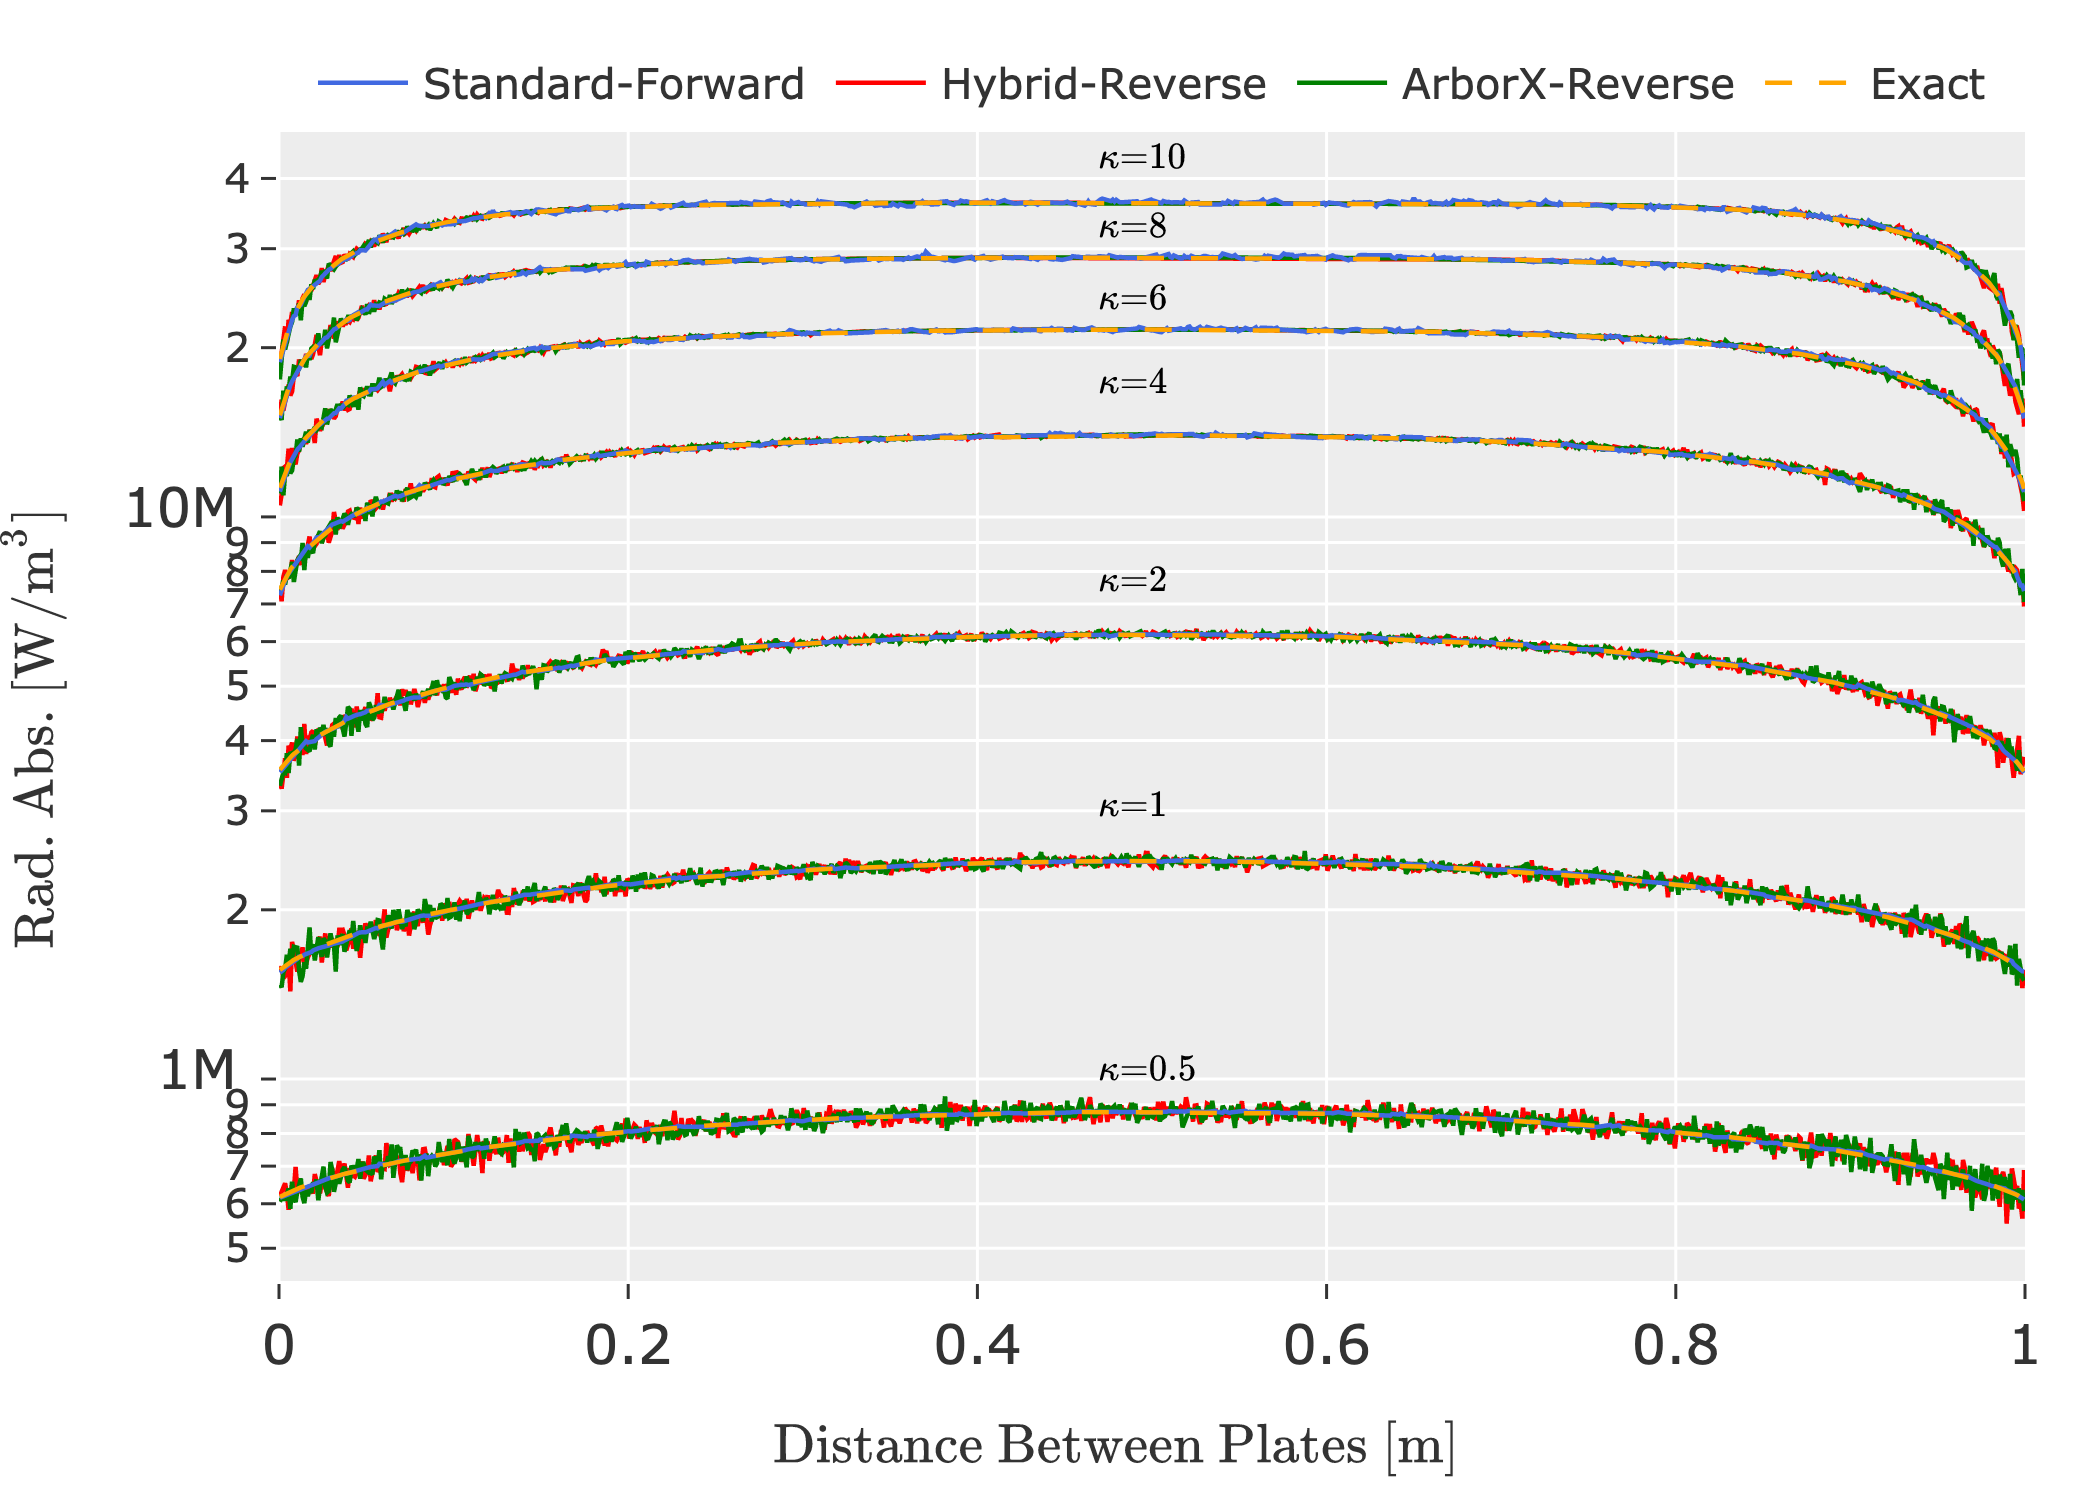
\includegraphics[width=\linewidth]{figures/ch4/PPcomparison1.png}
\caption{Variable absorption coefficient with T=$2000$K, N$_r$=$1000$, N$_{cells}$=1000.}
\label{fig:PPcomp_kappa}
\end{figure}

\begin{figure}
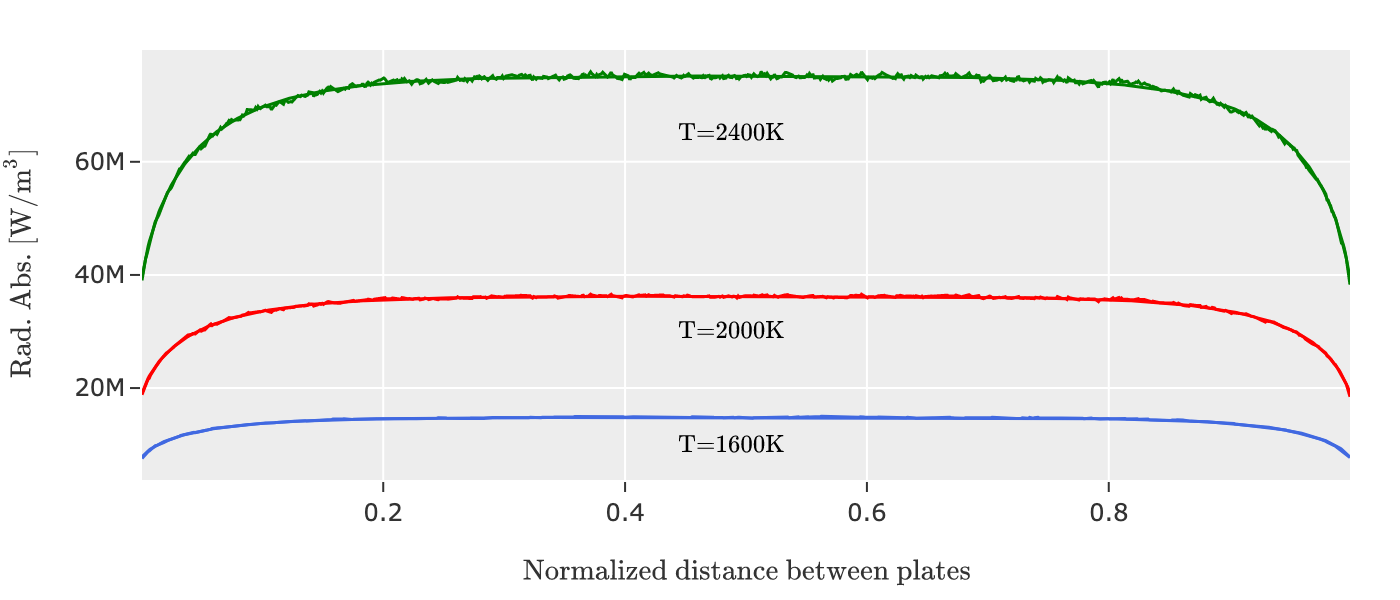
\includegraphics[width=\linewidth]{figures/ch4/PPcomparison2.png}
\caption{Variable temperature with $\kappa{}$=$10$ m$^{-1}$, N$_r$=$1000$, N$_{cells}$=1000.}
\label{fig:PPcomp_temp}
\end{figure}

\begin{figure}
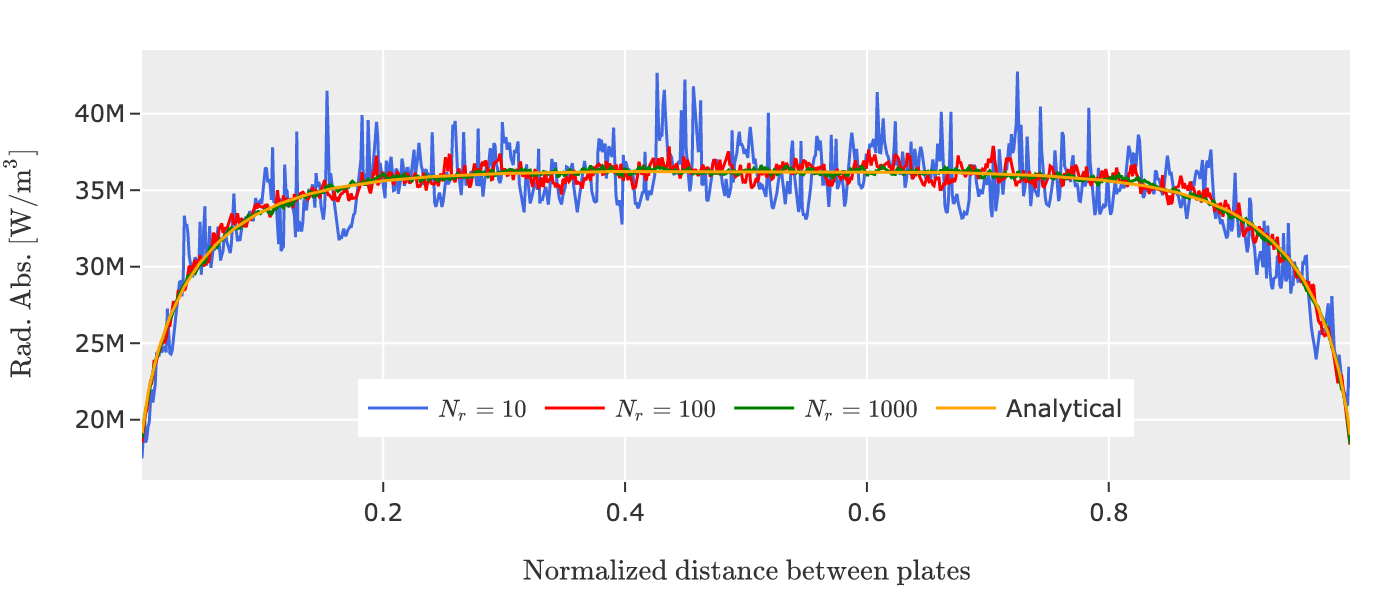
\includegraphics[width=\linewidth]{figures/ch4/PPcomparison3.png}
\caption{Variable number of rays emitted per cell (N$_r$) with $\kappa{}$=$10$ m$^{-1}$, T=$2000$K, N$_{cells}$=1000.}
\label{fig:PPcom_nrays}
\end{figure}

% \begin{figure}



%   \label{fig:PPcomp}
% \end{figure}

Results show excellent comparison between the MCRT and analytical implementations. 
The lower ray counts show a higher degree of variability resulting from the stochastic nature of the MCRT method. 
Increasing absorption coefficient leads in an increase of radiative emission and re-absorption, with re-absorption increasing at a higher rate resulting in a net increase of radiative source.

These expected results demonstrate the requirement for RTE modeling in optically thick media. Not only does radiative emission result in heat loss from computational cells, but also the re-absorption can be high enough to require modeling of the self-absorption process of radiation.

\section{Backward-Facing Step Combustor}
The backward-facing step (BFS) combustor is a convenient configuration often used as a simple, repeatable geometry for a variety of studies in fluid dynamics.
Numerous examples exist demonstrating its use for experimental and numerical investigations of turbulent flow~\cite{Armaly1983ExperimentalFlow,Neto1993AStep,Jovic1994Backward-facing5000,Le1997DirectStep}. In contrast, studies of combined turbulent and high temperature flow~\cite{Niemann2016Buoyancy-affectedNumber,Xie2017GeometrySteps}, and reacting flows~\cite{Pouech2021PremixedStep} over backward-facing steps have been modeled significantly less frequently.
In the relatively few studies that exist, the addition of volumetric heating and composition changes resulting from the exothermic chemical reactions have been shown to influence the flow patterns and turbulence intensity of the fluid. 
Recent interest has emerged regarding the relative influence of radiation and convection along the walls many configurations, and the backward-facing step geometry provides a convenient approach for doing so.

\subsection{Case setup}
\begin{figure}
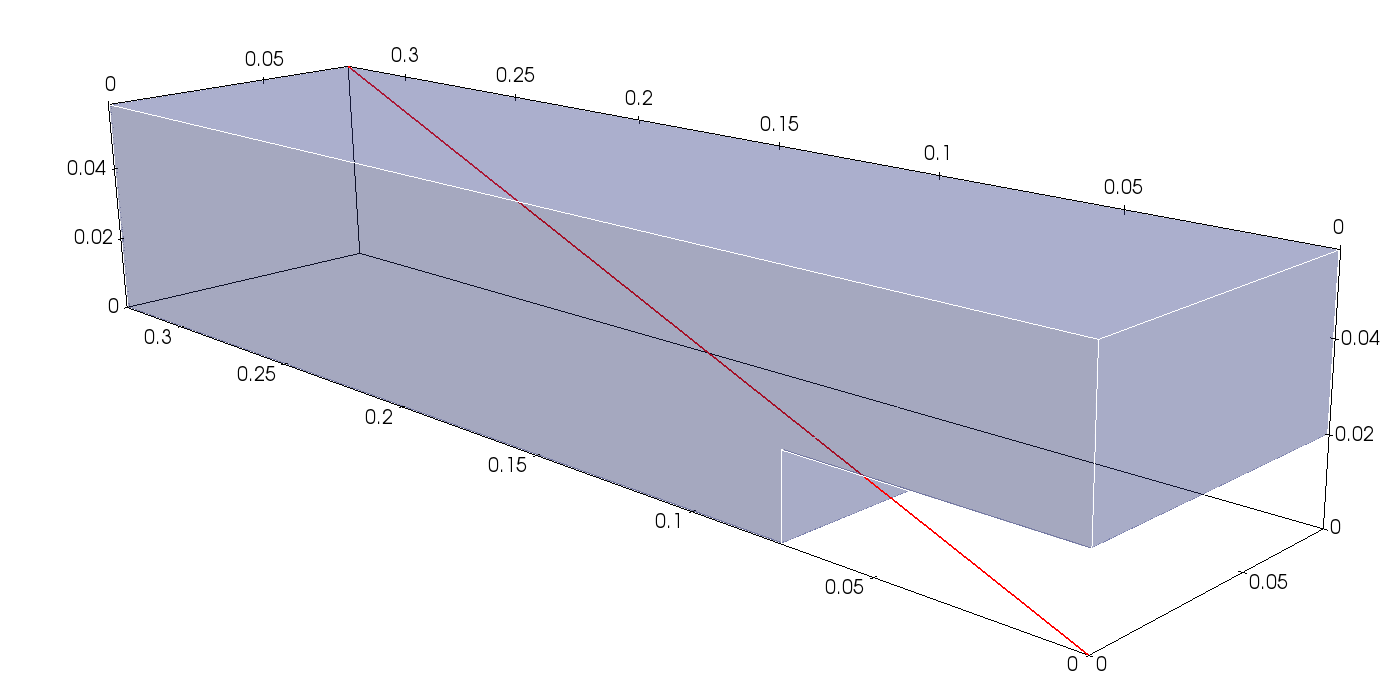
\includegraphics[width=\linewidth]{figures/ch4/BFS_visual.png}
\caption{Dimensions of backward-facing step configuration used in this study in addition to a representative line used to sample radiative properties. All units are in meters. }
\label{fig:BFS_geometry}
\end{figure}

CITE JULIANS THESIS

The BFS geometry used in this study is diagrammed in figure \ref{fig:BFS_geometry} based on an experimental configuration at the Pennsylvania State University.
A three-dimensional CFD calculation was performed closely matching the conditions present in the experiment. For this case, no chemically reacting flow is included. 
The flow is present in only vitiated form, where a chemical reaction is initiated in a portion of the flow upstream of the step, and the resulting "dirty" air with high CO$_2$ and H$_2$O content is mixed with unreacted air. 
The mixture reaches the main section at an elevated temperature of up to 850K, appreciably lower than expected temperatures of above 2000K when full reactions are present. 
The simulations account for the elevated temperature, but neglect any further chemical reactions beyond the step, resulting in a purely fluid-mechanical calculation.

Figures \ref{fig:BFS_temperature}, \ref{fig:BFS_streamlines} show temperature and velocity magnitude contours in the BFS. The pressure is atmospheric, and the absorption coefficient is assumed uniform at a value of 0.5 m$^{-1}$ due to the absence of chemical properties in the CFD simulations.

\begin{figure}

\end{figure}
\begin{figure}
  \begin{subfigure}{1\textwidth}
  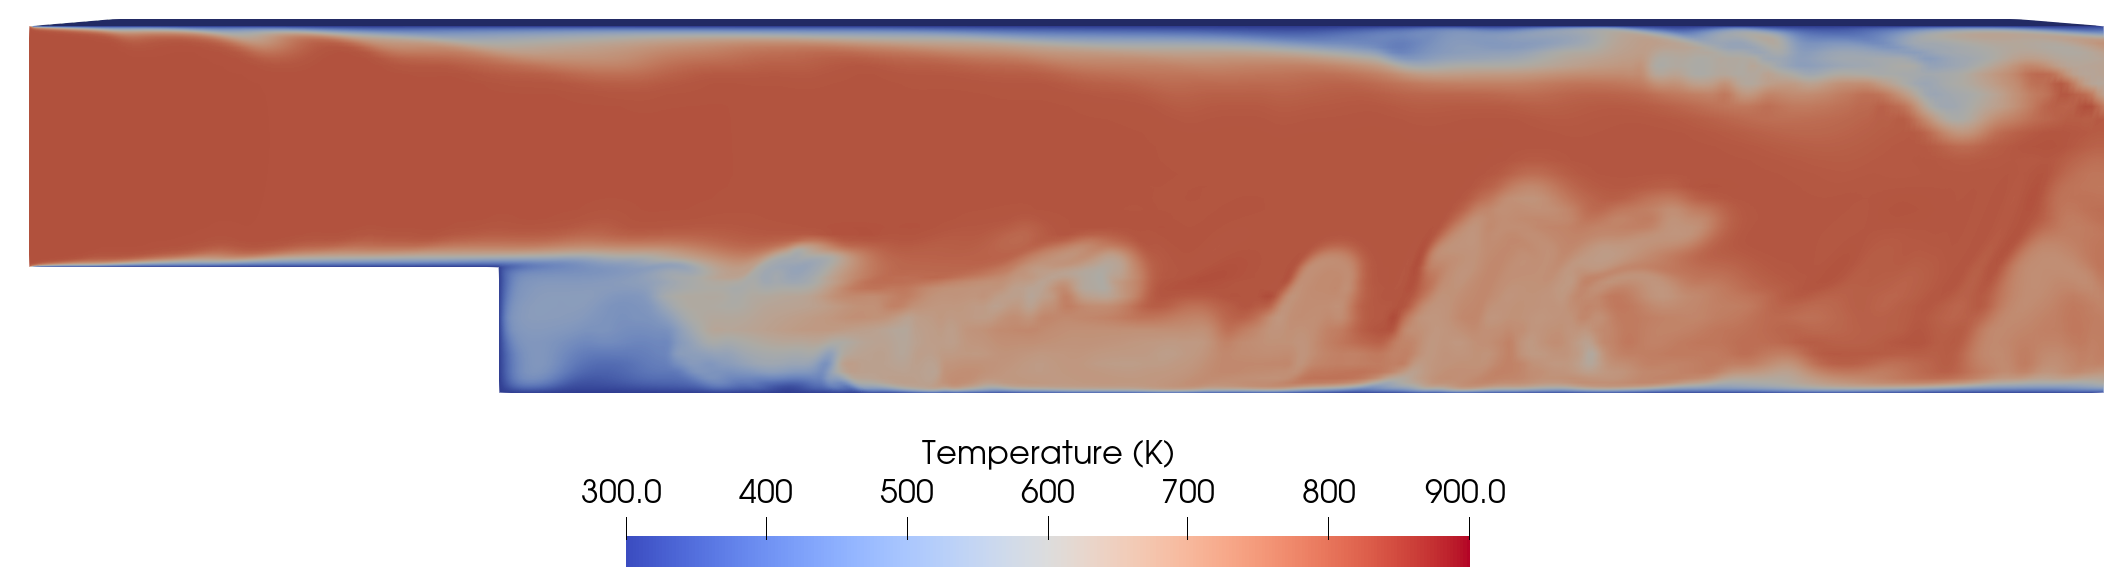
\includegraphics[width=\linewidth]{figures/ch4/BFS_temperature.png}
  \caption{BFS temperature contour along the mid-plane. }
  \label{fig:BFS_temperature}
  \end{subfigure}
  \begin{subfigure}{1\textwidth}
  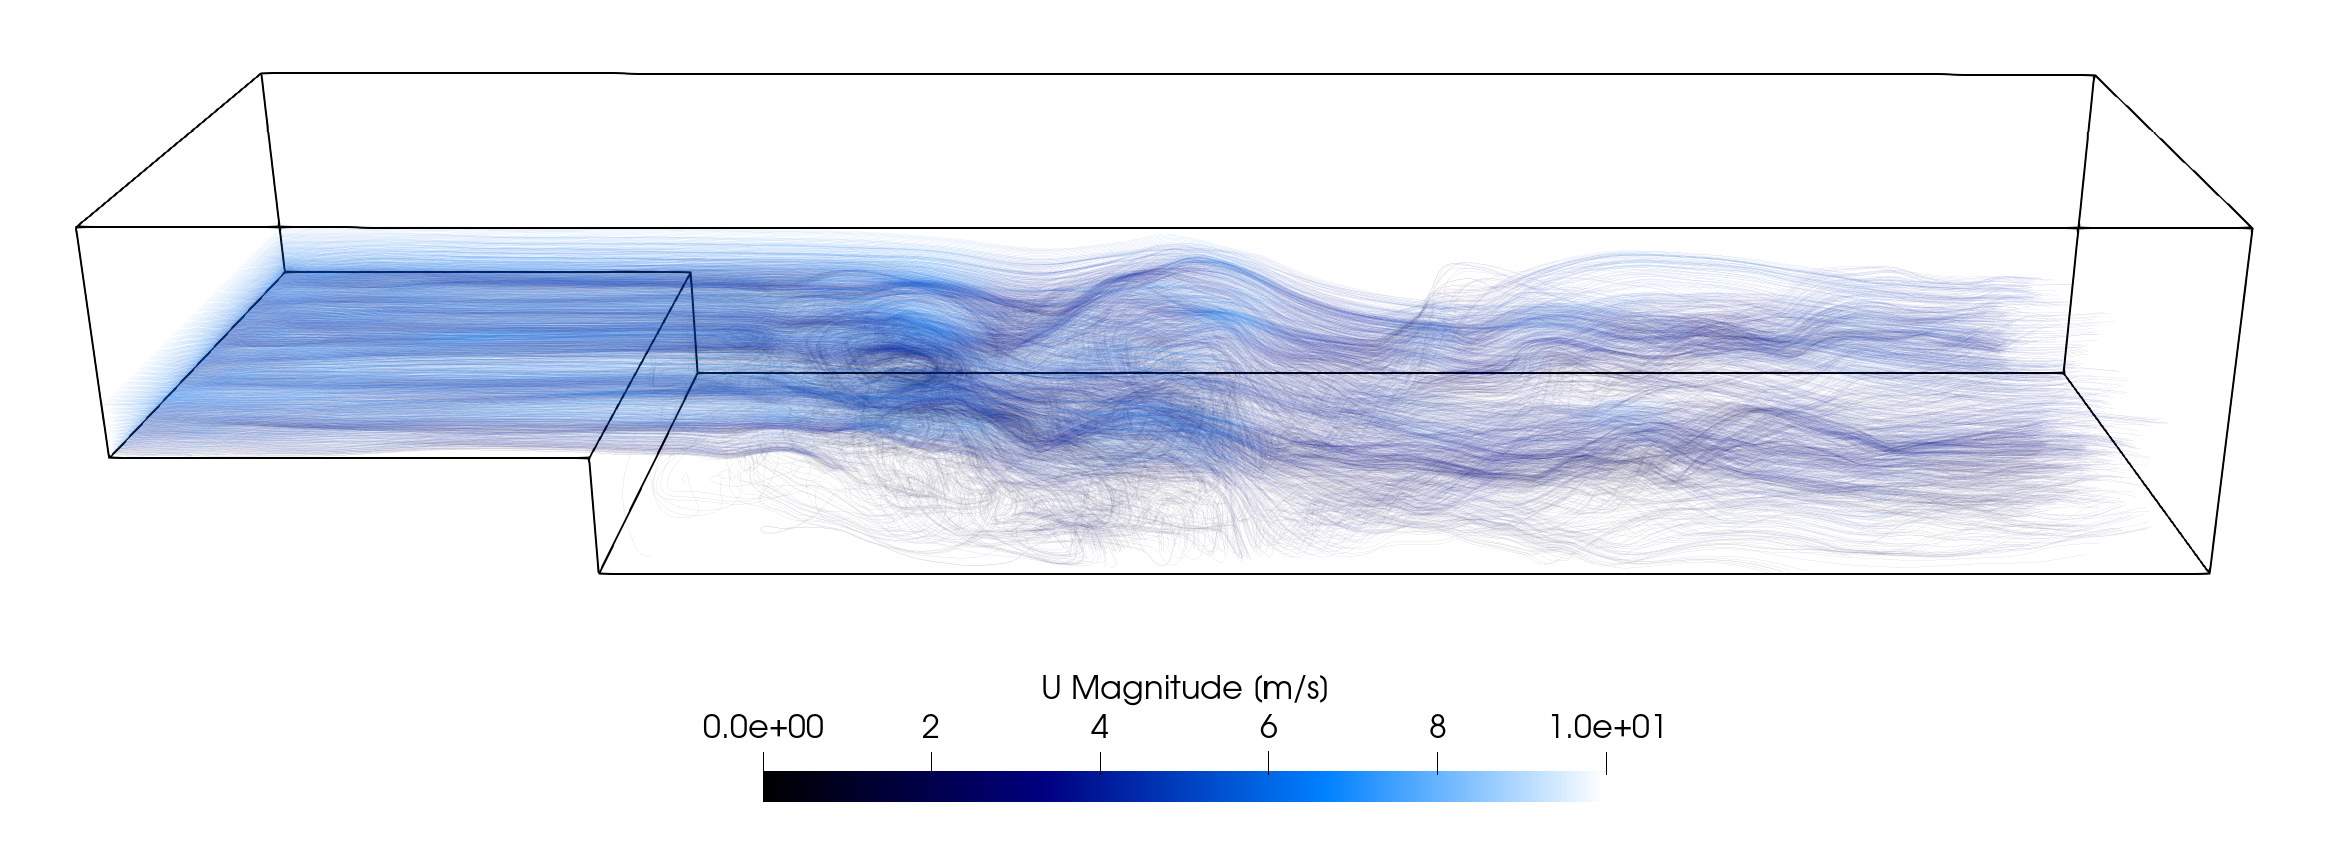
\includegraphics[width=\linewidth]{figures/ch4/BFS_streamlines6.png}
  \caption{Streamlines traced from the entrance of the BFS.}
  \label{fig:BFS_streamlines}
  \end{subfigure}
  \label{fig:BFS_contours}
\end{figure}

\subsection{Results}
A single time-step of the CFD simulation was extracted for a \textit{frozen field analysis} (see chapter \ref{chapter:Introduction}). 
The resulting radiative emission and wall-heat flux iso-contours are shown in figure \ref{fig:BFS_radiationcontours}.


\begin{figure}
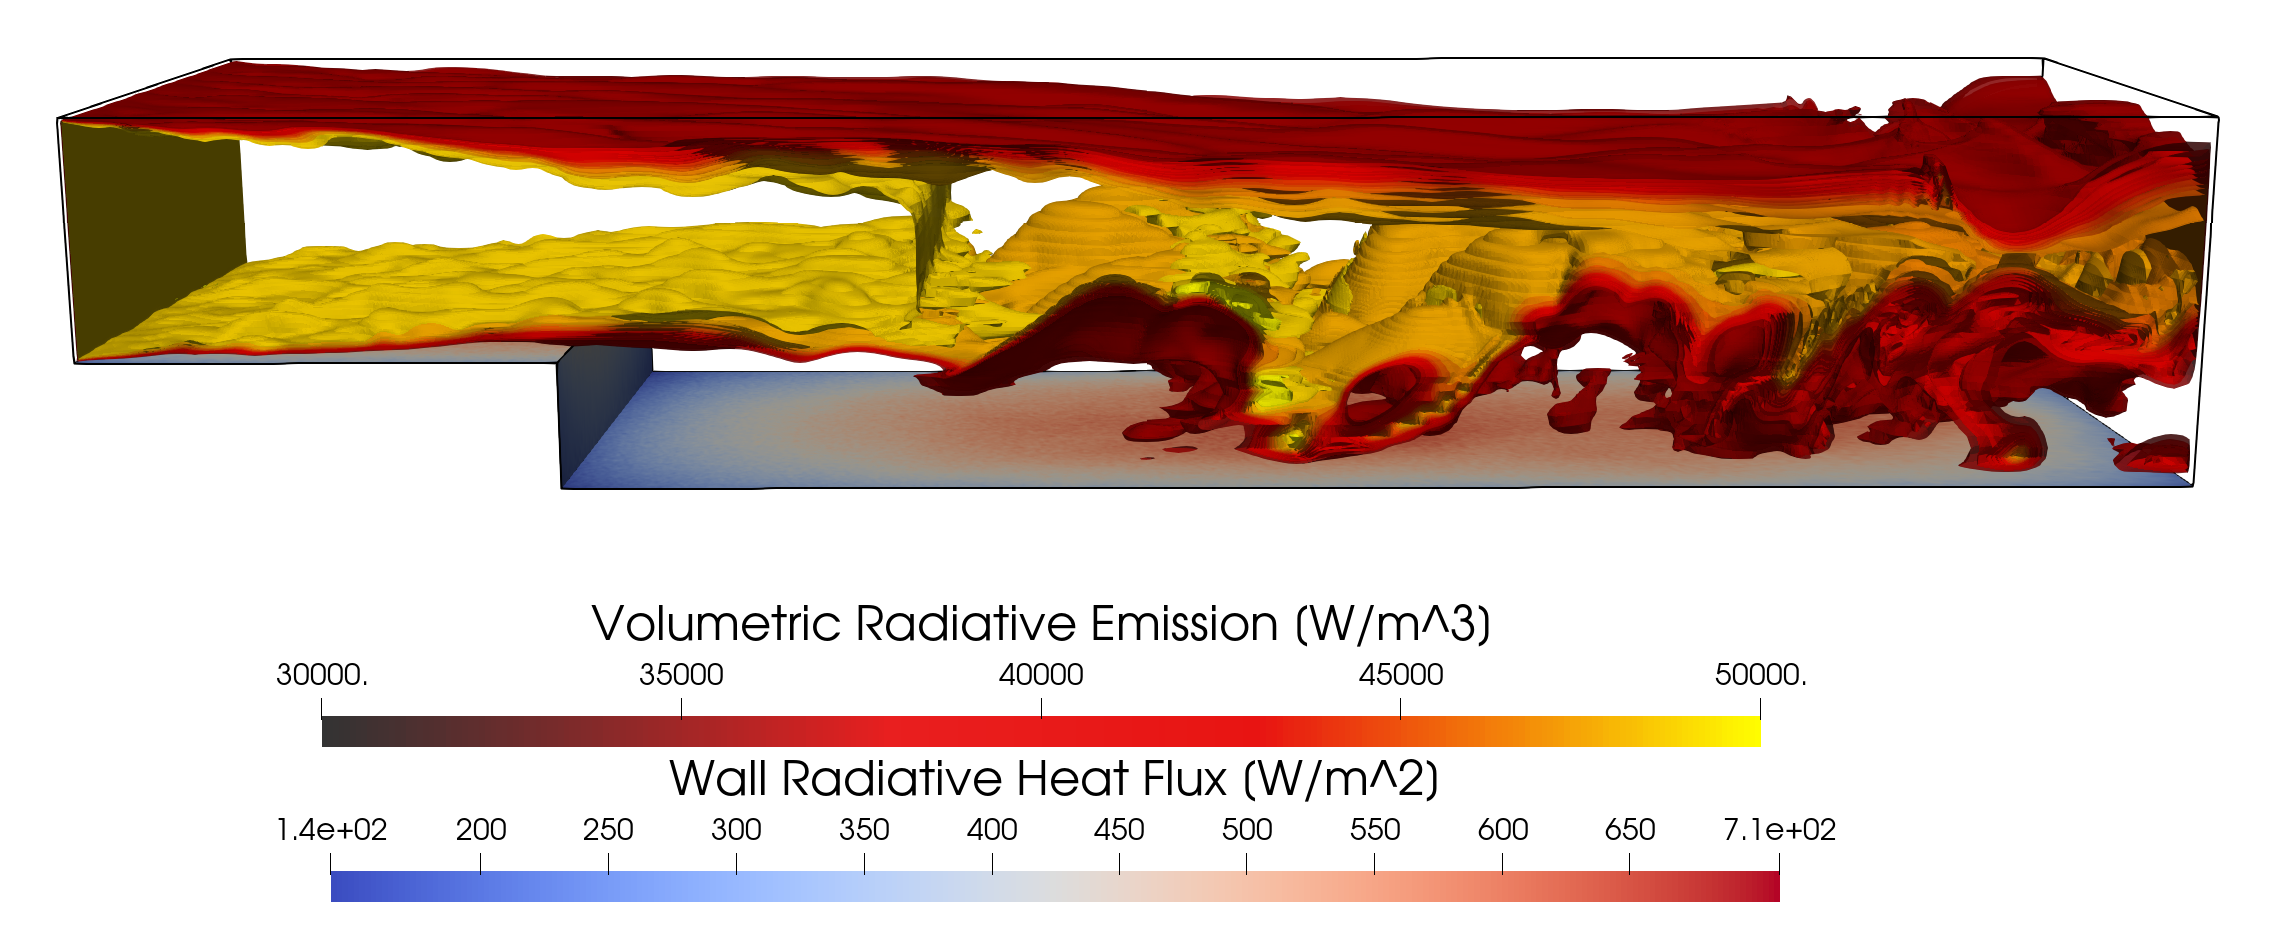
\includegraphics[width=\linewidth]{figures/ch4/BFS_volwallflux3.png}
\caption{Contours of volumetric radiative emission alongside resulting radiative heat flux along the walls.}
\label{fig:BFS_radiationcontours}
\end{figure}

The bulk of radiative emission originates from the re-circulation zone behind the step. Radiation is emitted from the flow and decreases the thermal energy contained in the passing fluid. 
The fluid is then quickly replaced by the new gas at the entrance, which results in a continuous load of radiation incident on the bottom surface of the domain. 

The turbulence present in the recirculation zone is apparent even in the emission contours as a result of the advection of elevated temperatures present. The secondary recirculation zone immediately present adjacent to the step displays lower levels of radiative emission resulting from its slower rate of fresh-gas replenishment.

Figures \ref{fig:BFS_RadAbs}, \ref{fig:BFS_RadEmi}, and \ref{fig:BFS_RadSrc} show the radiative absorption, emission, and net energy source along the line shown in figure \ref{fig:BFS_geometry} using the different solvers for comparison. 

\begin{figure}[!ht]
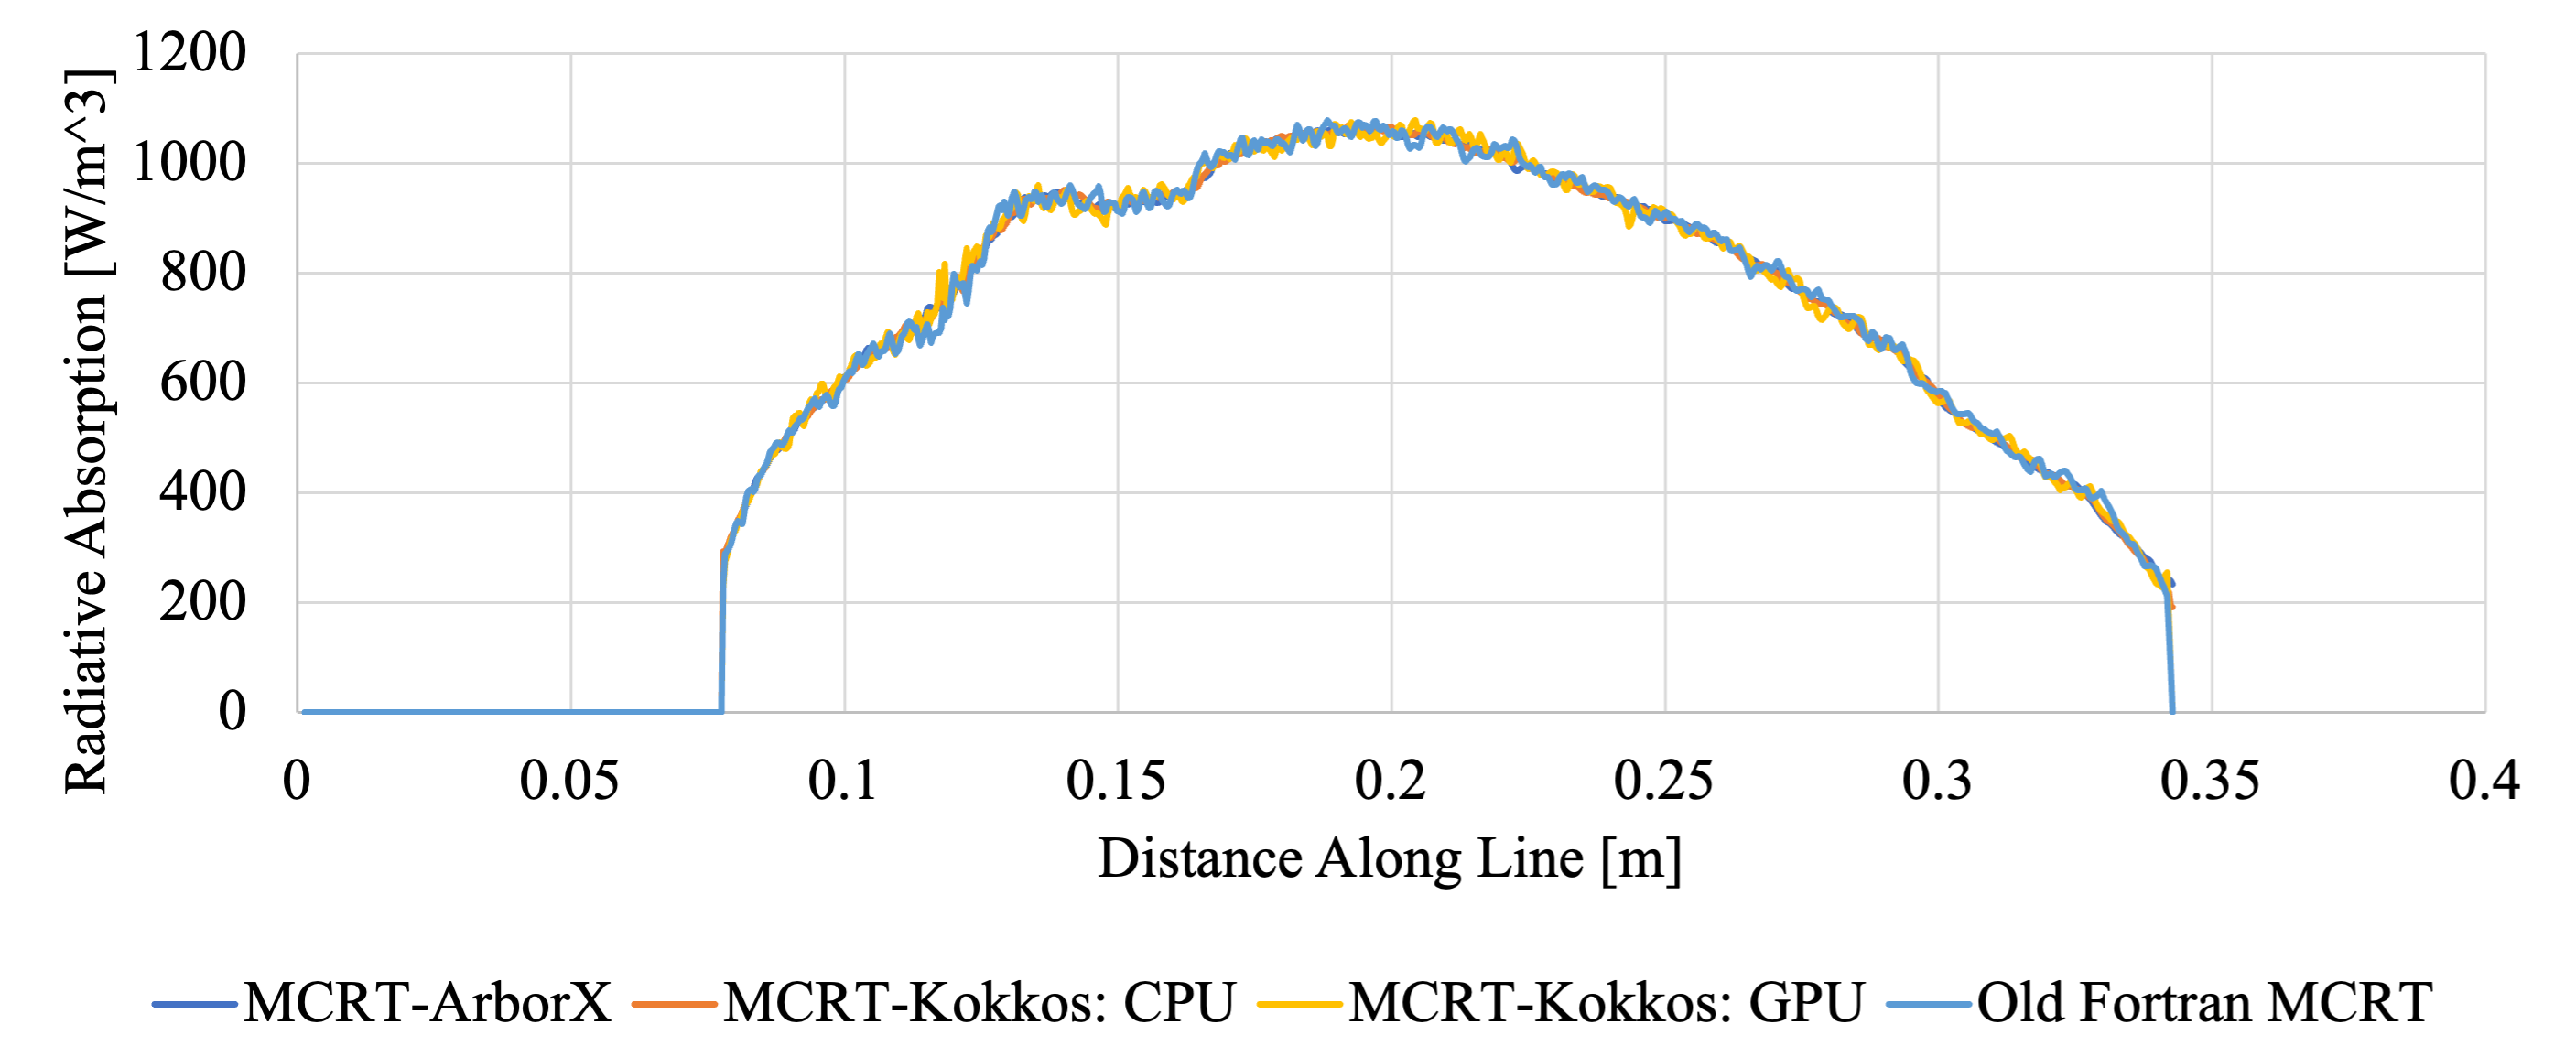
\includegraphics[width=\linewidth]{figures/ch4/LineComparison_RadAbs.png}
\caption{}
\label{fig:BFS_RadAbs}
\end{figure}

\begin{figure}[!ht]
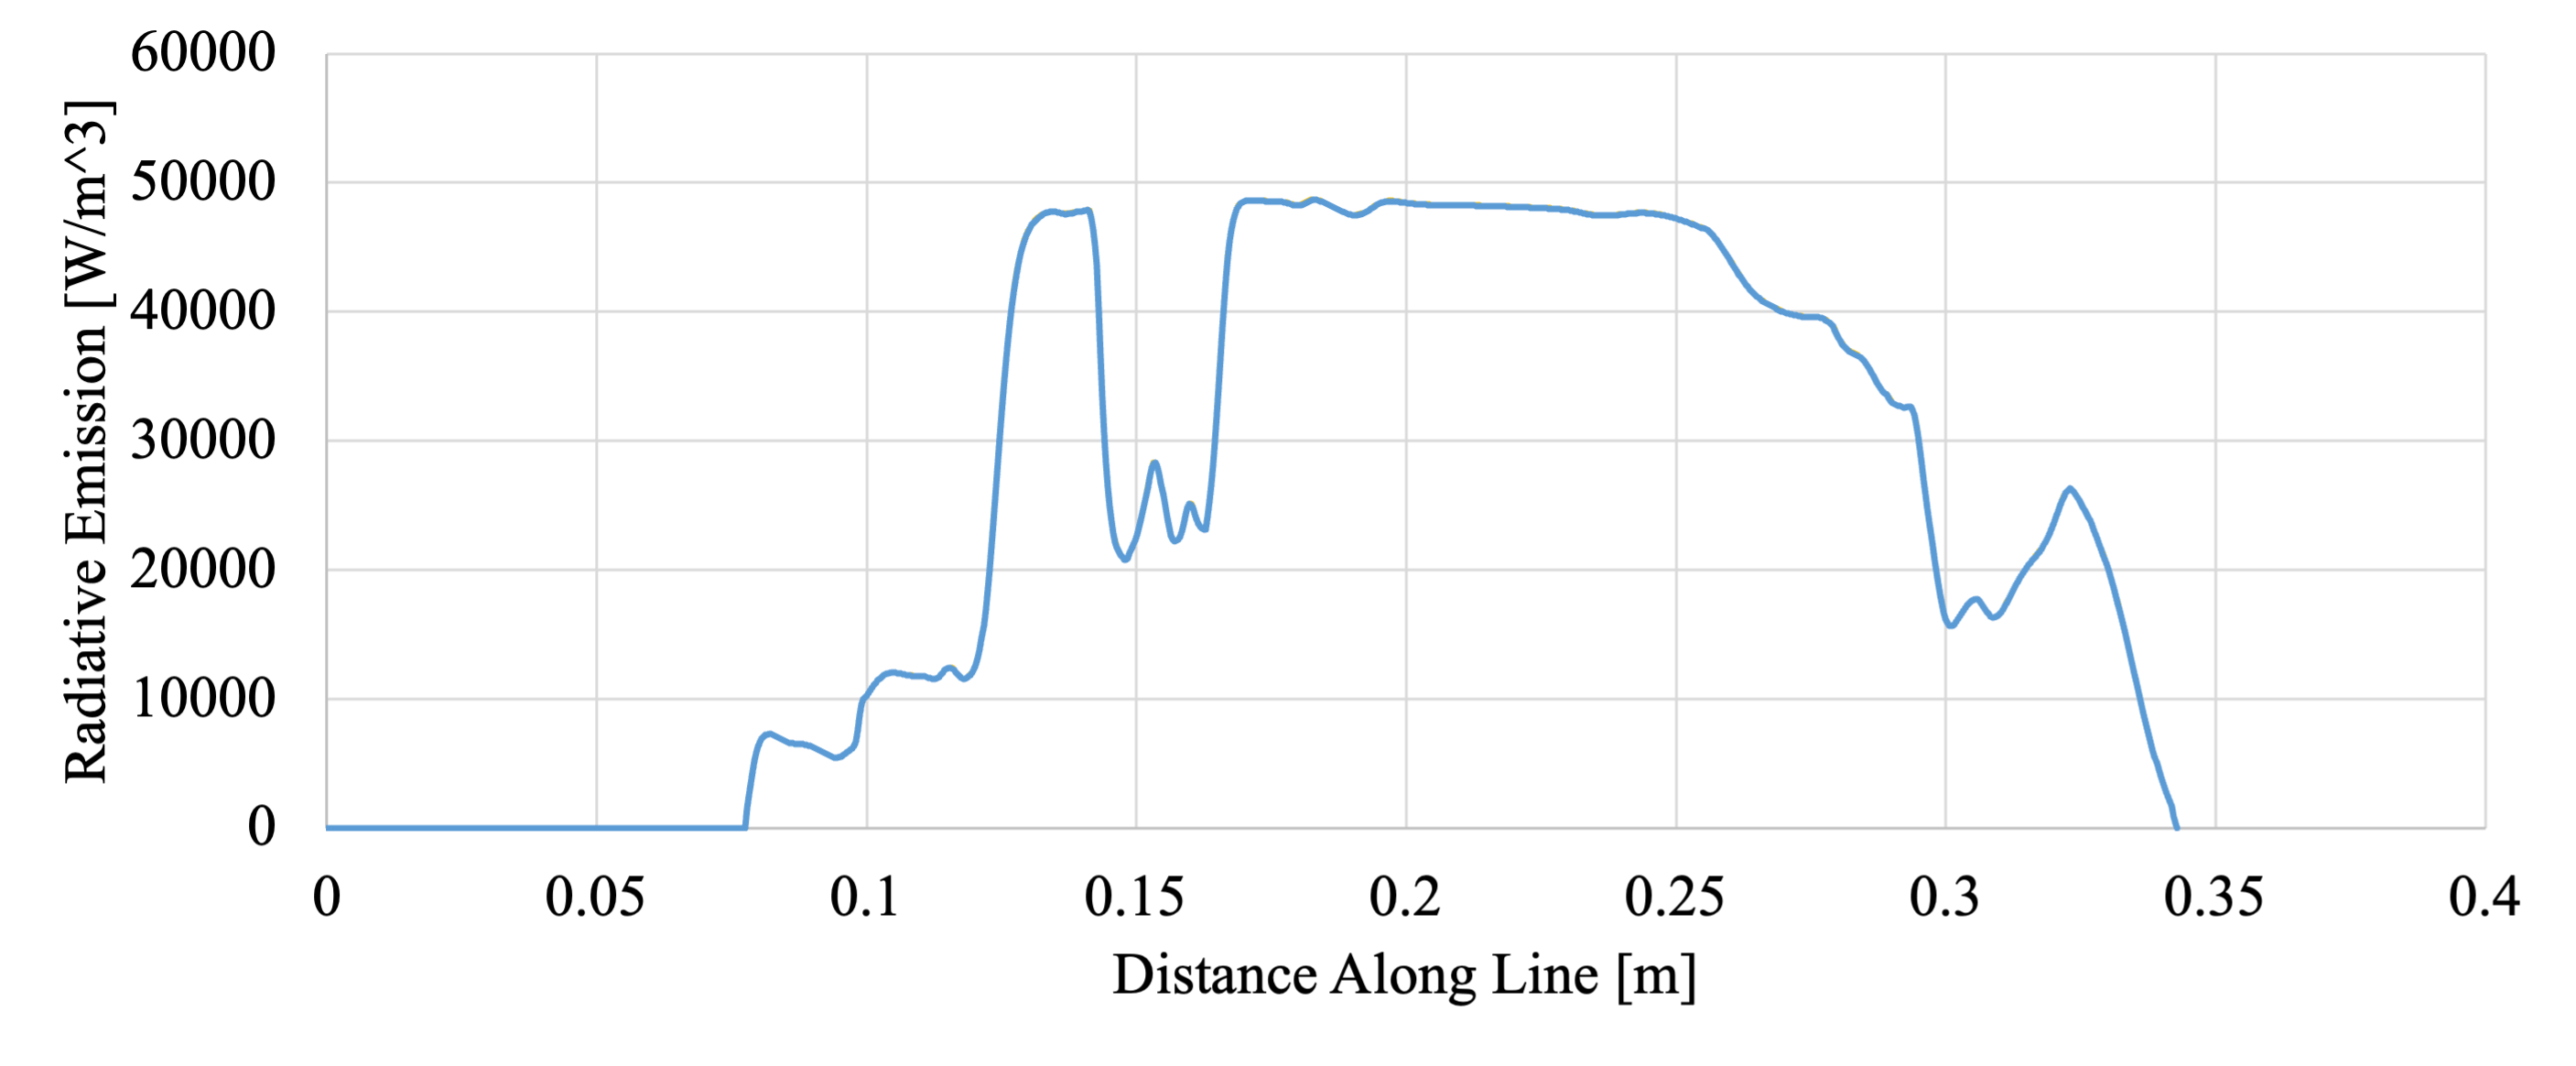
\includegraphics[width=\linewidth]{figures/ch4/LineComparison_RadEmi.png}
\caption{Note: Same legend as in fig. \ref{fig:BFS_RadAbs}. All results overlap exactly.}
\label{fig:BFS_RadEmi}
\end{figure}

\begin{figure}[!ht]
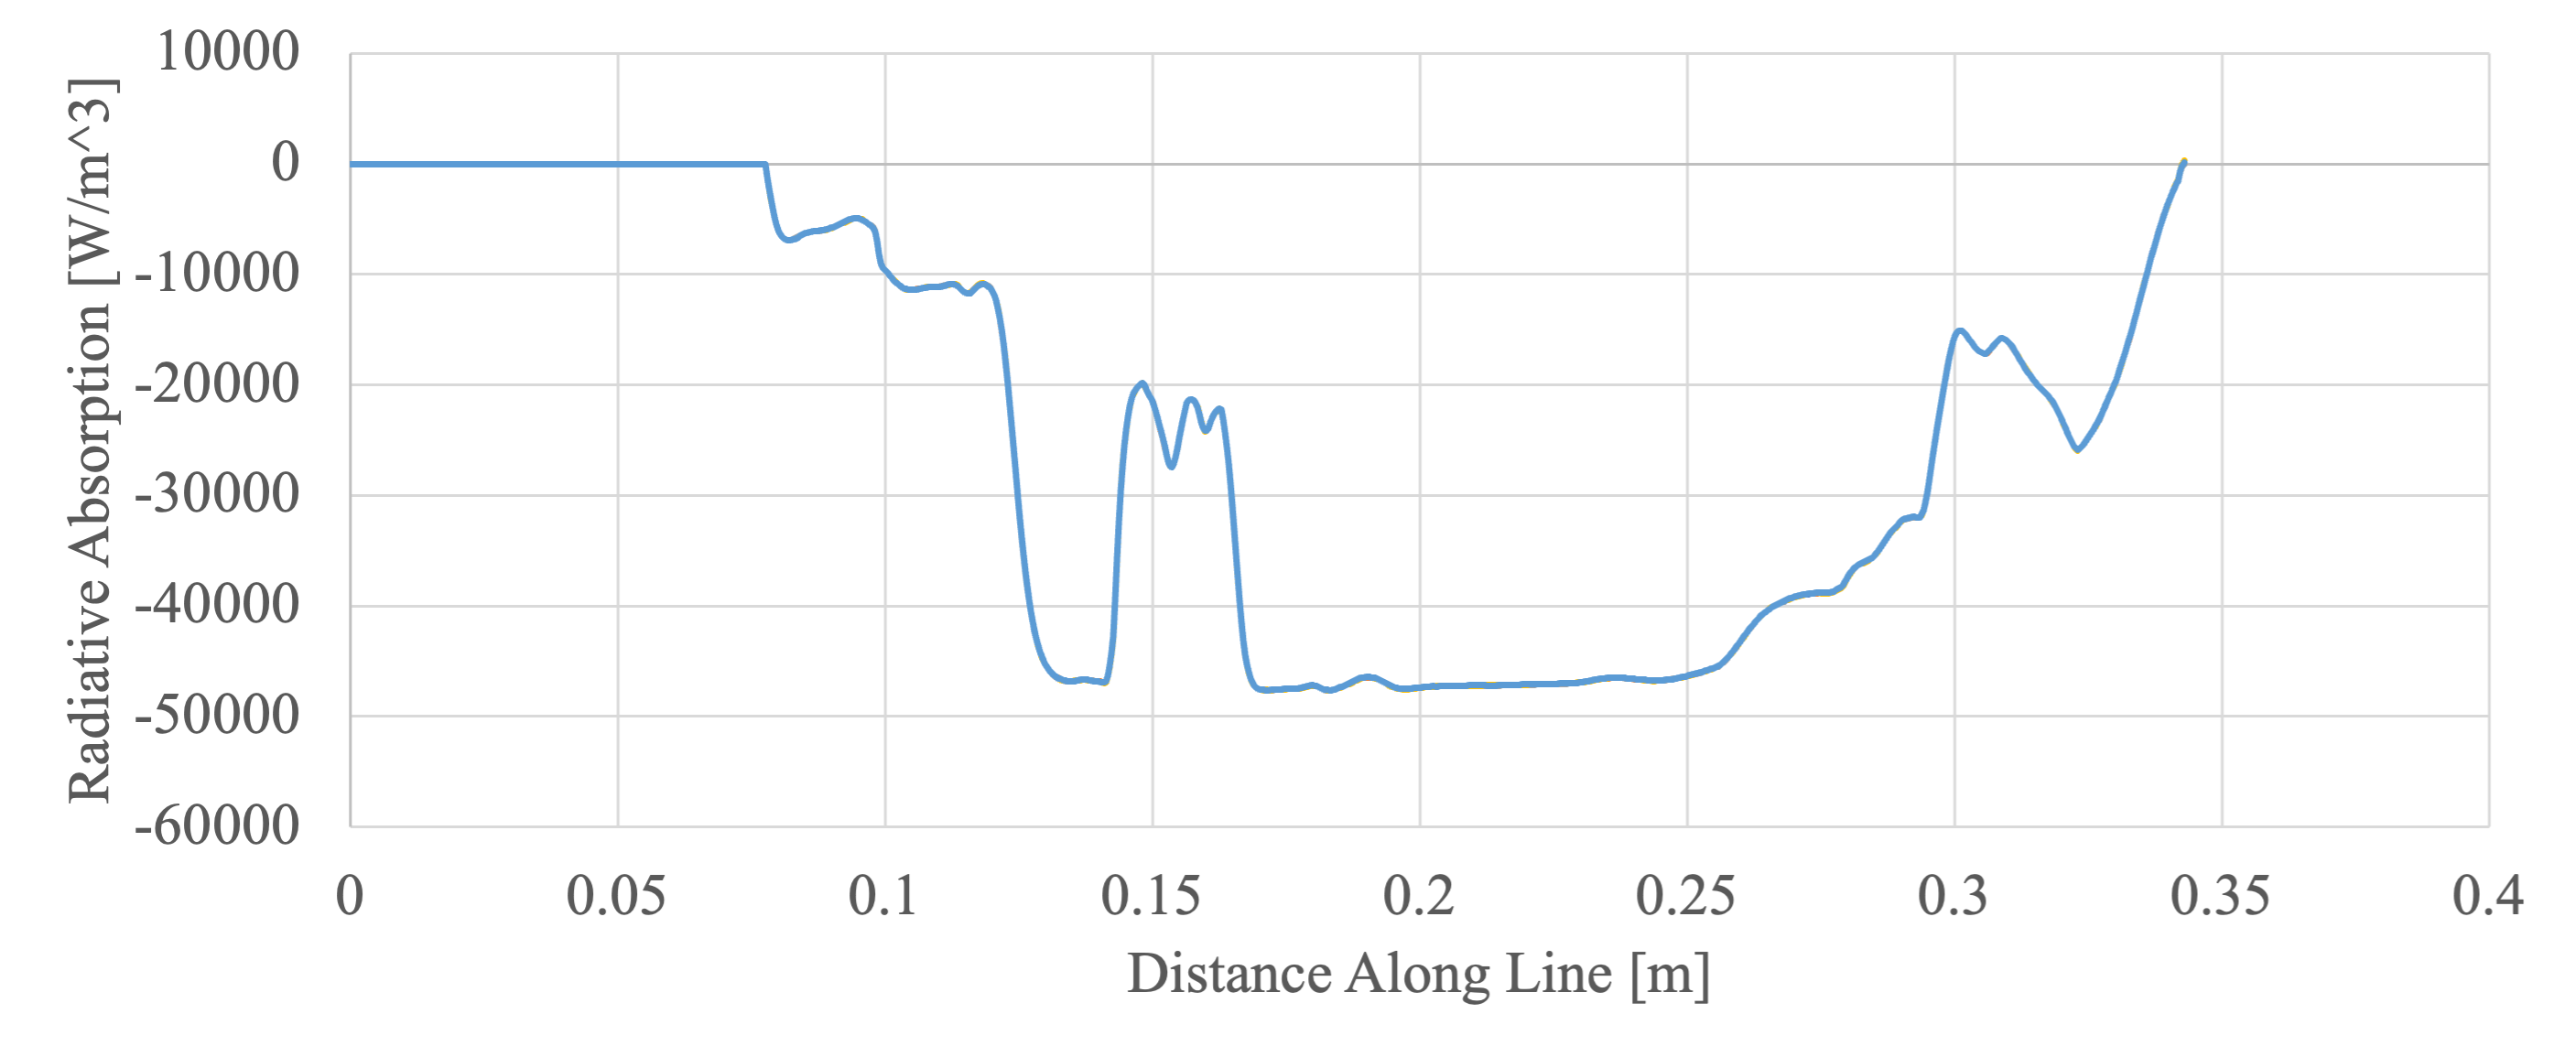
\includegraphics[width=\linewidth]{figures/ch4/LineComparison_RadSrc.png}
\caption{Note: Same legend as in fig. \ref{fig:BFS_RadAbs}. All results overlap exactly.}
\label{fig:BFS_RadSrc}
\end{figure}


\subsection{Model Performance}
The radiation was calculated using both new MCRT models as well as a well-established Fortran-based radiation model for comparison. Simulations were performed at the single time-step using both 1 ray per cell and 10 rays per cell for all solvers, and serial, OpenMP and Cuda were tested as Kokkos backends for the new MCRT. 
Simulations were performed using a 72-core Intel(R) Xeon(R) Gold 5220 CPU shared-memory workstation for OpenMP calculations, and Cuda calculations were performed using NVIDIA V100 GPUs from the high performance computer Narwhal operated by the defense super-computing resource center~\cite{something}.

Results are listed in tables \ref{table:BFS_runtime_table_1rpc} and \ref{table:BFS_runtime_table_10rpc} for 1 ray emitted per cell and 10 rays per cell, respectively. The performance of both the MCRT-Kokkos model and the MCRT-ArborX compare extremely well against the MCRT-Fort model for a serial calculation. A runtime improvement of 86\% is already observed before any parallel routines have even been applied.
The dramatic speedup can be attributed to the improved mesh-transfer method implemented in the new MCRT methods. 
Almost no mesh data is duplicated during the mesh transfer process, allowing for minimal delay before the raytracing procedure begins. VERIFY THIS AND COMPARE WITHOUT THE MESH TRANSFER. WHY DOES SERIAL RUN OVER 50X FASTER THAN 30 PROCS?

\begin{table}[h!]
\centering
\begin{tabular}{||c c c c||} 
 \hline
 Parallel Variation & MCRT-Fort & MCRT-Kokkos & MCRT-ArborX \\ [0.5ex] 
 \hline\hline
 Serial & 2687 s & 376 s & - \\ 
 30 CPU Processors & 52.26 s & 22.5 s & - \\
 GPU & N/A & 6.91 s & - \\
 \hline
\end{tabular}
\caption{BFS runtime comparisons with 1 ray emitted per CFD cell. The MCRT-Fort parallel procedure is conducted using separate MPI processes within a shared-memory system. The MCRT-Kokkos and MCRT-ArborX run using 30 OpenMP processes.}
\label{table:BFS_runtime_table_1rpc}
\end{table}

\begin{table}[h!]
\centering
\begin{tabular}{||c c c c||} 
 \hline
 Parallel Variation & MCRT-Fort & MCRT-Kokkos & MCRT-ArborX \\ [0.5ex] 
 \hline\hline
 30 CPU Processors & 504.37 s & 197.6 s & - \\
 GPU & N/A & 49.1 s & - \\
 \hline
\end{tabular}
\caption{BFS runtime comparisons with 10 rays emitted per CFD cell.}
\label{table:BFS_runtime_table_10rpc}
\end{table}


The introduction of a parallel CPU implementation also results in dramatic speedups for all three MCRT implementations. MCRT-Fort sees a large speedup not only due to its parallel ray-tracing procedure, but also the long time required to initialize the mesh is reduced resulting from the 30 MPI processes used\footnote{OpenFOAM will load different sections of the mesh on different processors simultaneously when MPI parallelism is used. In this case, the MCRT-Fort code has only been enabled to use MPI parallelism.}.
Within MCRT-Kokkos and MCRT-ArborX, runtimes are decreased as well, but to a lower extent. This can be attributed to the longer mesh initialization time resulting from the usage of a single MPI process.

The usage of a GPU enabled a significant reduction in runtime as well. 


\section{Small Pool Flame}
The emission of radiation from a buoyant pool flame is of considerable interest to those in the field of fire research. 
The relatively slow fluid motion alongside buoyancy-driven turbulent fluctuations provides a realistic surrogate for many hazardous combustion scenarios such as forest fires and house fires.
The high temperatures from the chemical reaction alongside the larger length scales also provide conveniently high radiative emissions alongside high optical thicknesses. 
This results in a system with a high degree of radiation, and is therefore a convenient sample case to demonstrate the use of the present radiation model.

\subsection{Case Setup}
The simulation is based on the fireFoam tutorial case, smallPoolFlame3D in \verb|OpenFOAM|, where mesh refinement has been doubled. 
In the tutorial case, a mass-source is provided through the inlet at the bottom of the domain, where a reaction is initiated. A turbulent premixed flame is then simulated with infinitely-fast chemistry for four seconds of physical time.
The simulation is run with radiation enabled, where the net radiation source terms are added to the CFD energy equation solution every timestep.
Both a frozen-field analysis and a full time-accurate simulation are conducted. Figure \ref{fig:PoolFire_diagram} displays the timestep for the former.

The geometry is a cubic 1$\times$1$\times$1m domain with a grid consisting of 1,728,000 hexahedral cells with 120 divisions per side.
10 rays are emitted and traced from each cell, irrespective of cell emission energy.
This configuration is studied for both planck-mean gray and line-by-line spectral models, and no Turbulence-Radiation Interaction (TRI) is accounted for in this study.

\begin{figure}
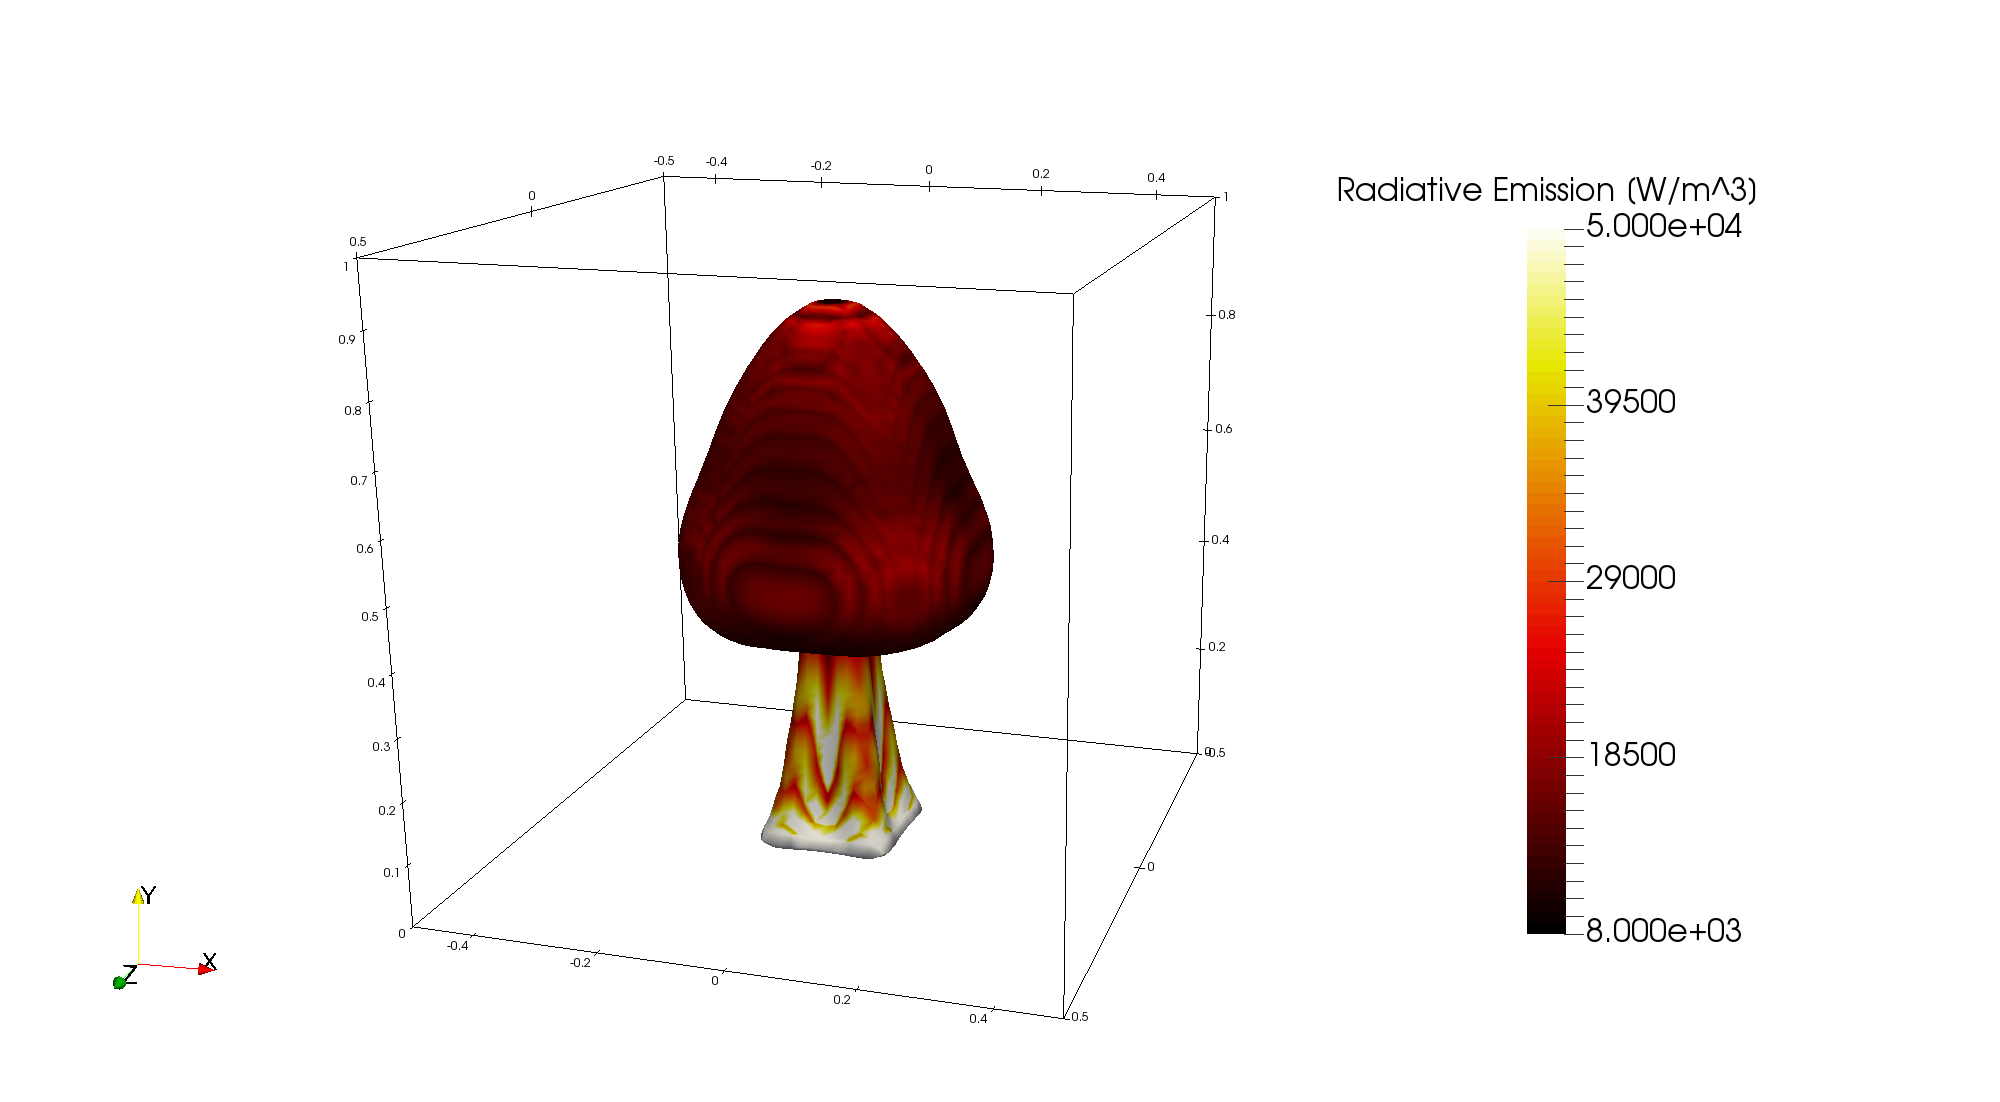
\includegraphics[width=\linewidth]{figures/ch4/contour_early.png}
\caption{An early timestep of the pool fire flame simulation. Isosurface is 0.03 CO$_2$ mass fraction colored by velocity magnitude in meters per second. Axes dimensions are in meters.}
\label{fig:PoolFire_diagram}
\end{figure}

\subsection{Results}
Figure \ref{fig:PoolFire_radiationcontours} displays the radiative emission and wall absorption patterns for the flame. Wall heat flux is maximized near the inlet section, directly adjacent to the location of ignition. 
The radiative emission contours drop towards the outer edges and top section of the mushroom-like shape. The turbulent mixing of the reacting flow with surrounding quiescent fluid results in a reduction in temperature, and lower volumetric emission.  

\begin{figure}
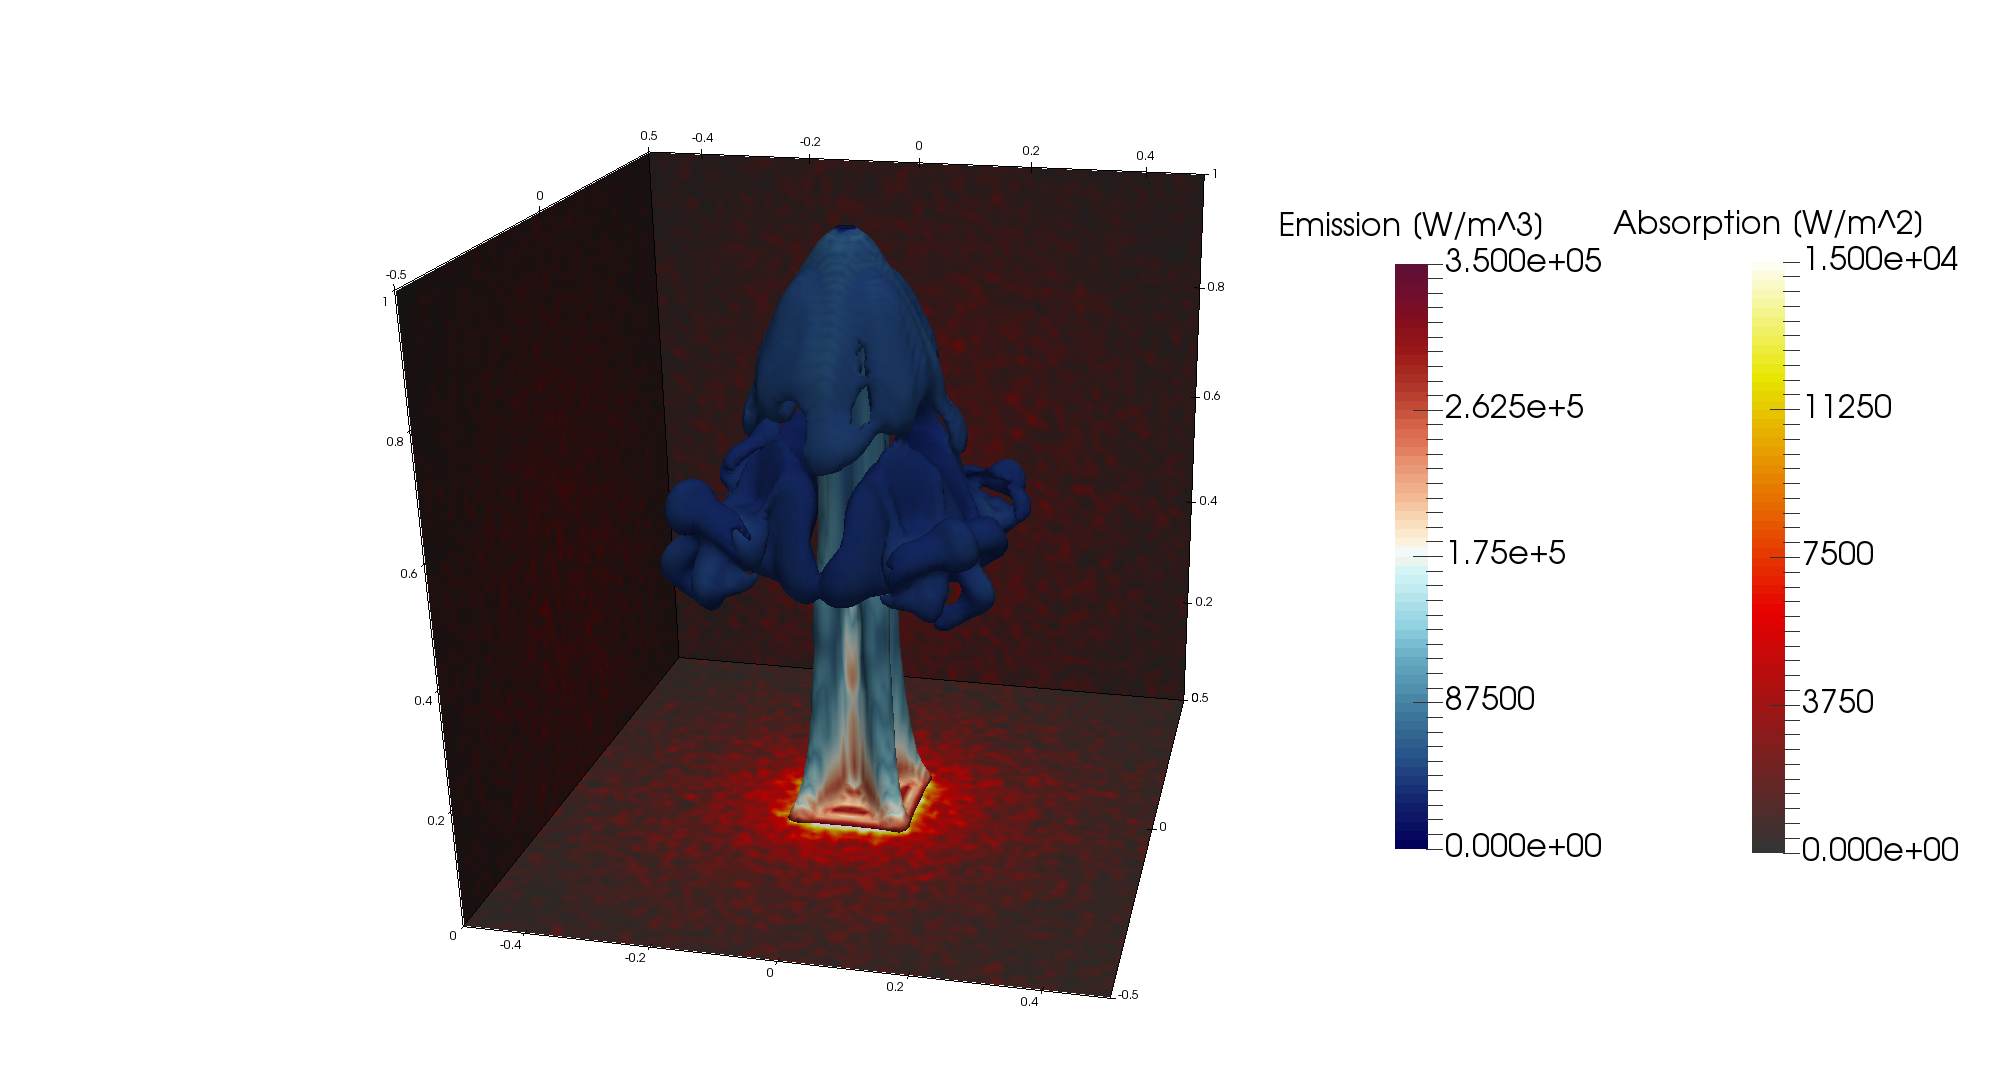
\includegraphics[width=\linewidth]{figures/ch4/radiation_contours.png}
\caption{Isosurface of 0.03 CO$_2$ mass fraction colored by radiative emission. Wall coloring represents wall radiative heat flux.}
\label{fig:PoolFire_radiationcontours}
\end{figure}

\subsubsection{Frozen field analysis}

In order to better understand the influence of radiation within the flame, figure \ref{fig:PoolFire_quadcomparison} displays four relevant parameters for the radiation calculation within the frozen field analysis. 
The contours of temperature show two sides of a hollow cylinder of reacting flow billowing upwards as a result of the buoyant force induce on the lower-density regions.
The top-section of the mushroom contains an  flame-front which, towards the outer regions, slowly decreases in temperature and intensity as a result of momentum and molecular exchange with the surrounding quiescent region through viscous and diffusive effects.
High temperature regions correlate strongly with the points of high emission, and the wings of the mushroom show a much stronger decay in emission as a result of the fourth power dependence of radiative emission with temperature.

Absorption visually appears to correlate much more closely with the Planck-mean absorption coefficient than temperature. Absorption is maximized near the entrance region of the flame, and maintains its strength throughout the tight upwards-moving stream of fluid.
The significant drop in Planck-mean absorption coefficient with radiative absorption in the non-reacting regions of the flow suggests that the flame is responsible for the bulk of radiative re-absorption. 

In total, net radiative emission equals $10541.5044$ Watts, where $1469.4406$ Watts are re-absorbed into the medium, and $9072.0639$ Watts escape to the walls. This results in approximately 14\% of radiative emission being re-absorbed primarily in the flame-region, as suggested previously. 
The maximum volumetric radiative energy loss for any computational cell is -$1.081$ W. In comparison, the maximum volumetric source through chemical reaction was $14.08$ Watts.

\begin{figure}
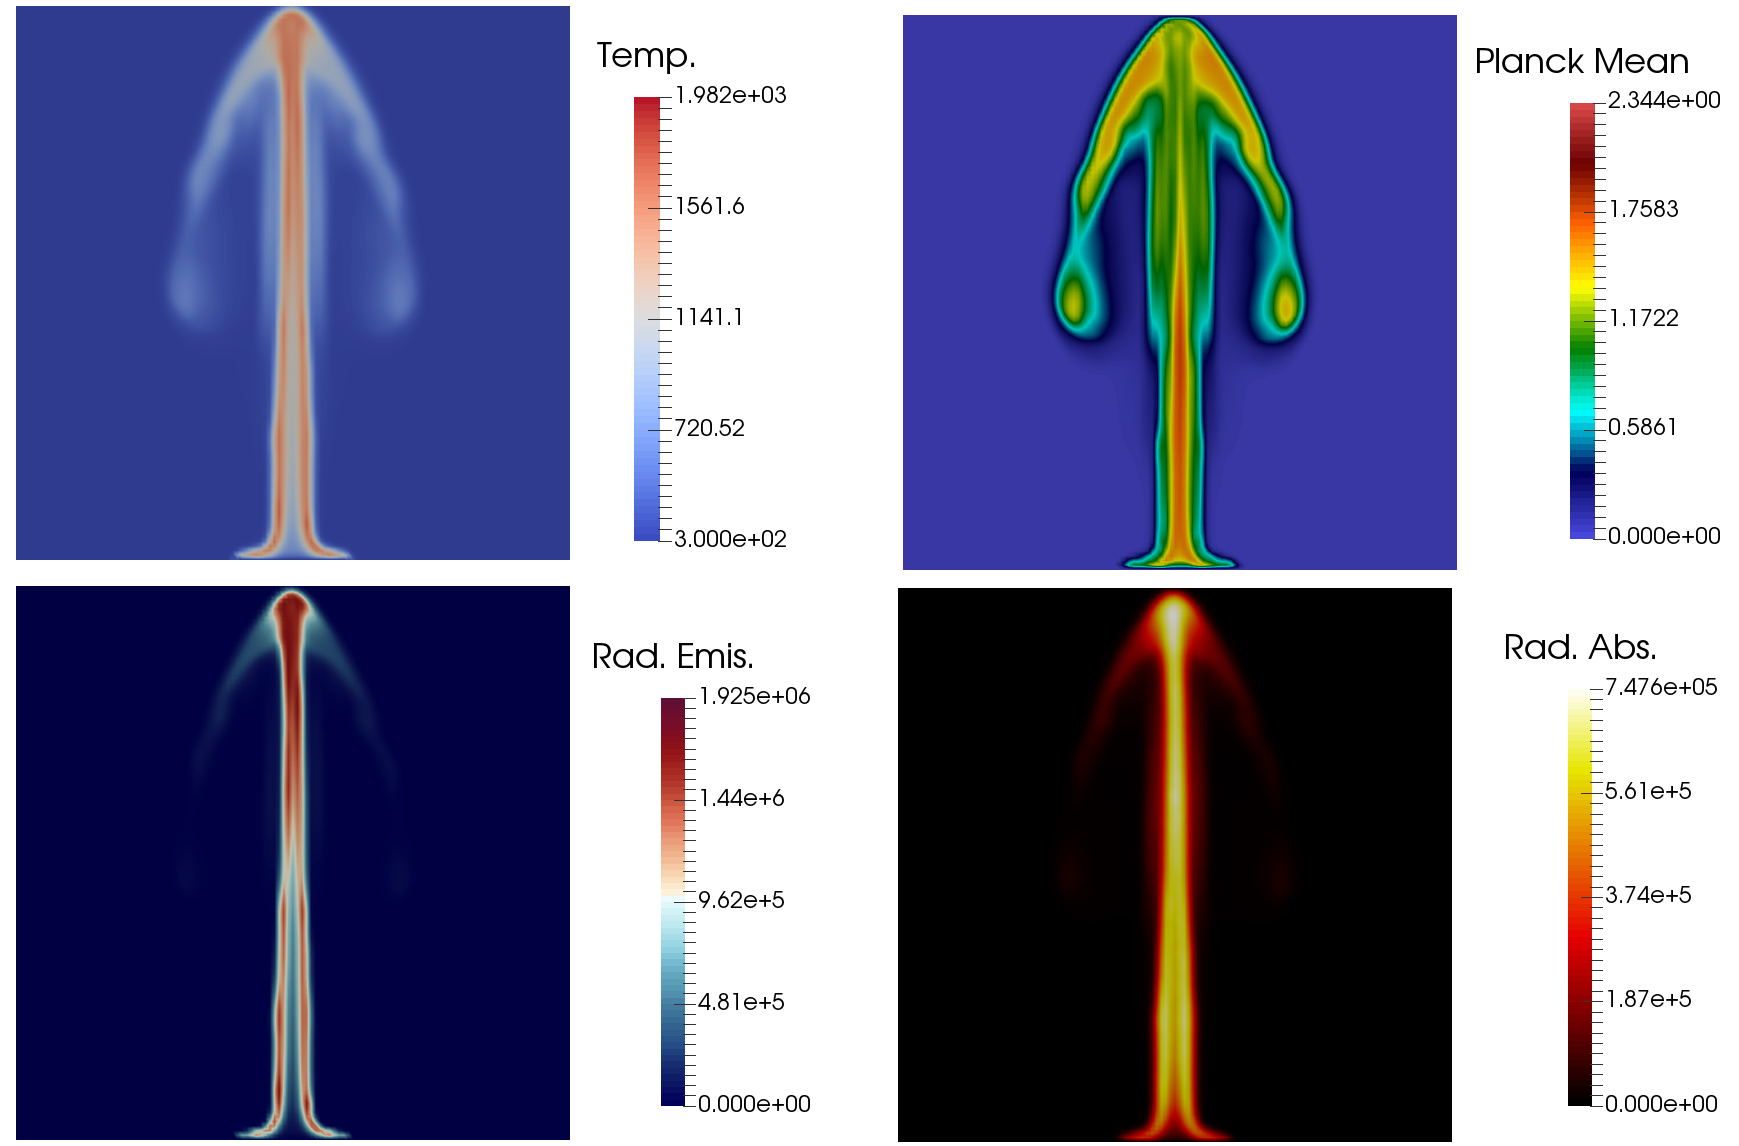
\includegraphics[width=\linewidth]{figures/ch4/PoolFire_quadcomparison.png}
\caption{Mid-plane contours of four relevant parameters to the radiation calculation in the pool fire.}
\label{fig:PoolFire_quadcomparison}
\end{figure}

Figure \ref{fig:PoolFire_lineplot} shows various normalized parameters along the center-line of a gray-simulated flame. 
Normalized temperature and product species mass fractions rise with increasing distance from the bottom surface, indicating reaction progression. 
The volumetric emission and negative of radiative volume source (emission – absorption) appear to match as a result of the relatively weak influence of absorption.
The Planck Mean absorption coefficient increases, then decreases despite the monotonically increasing mass fractions of the radiatively participating species (CO$_2$ and H$_2$O). This happens as a direct result of the increase in temperature. 
The influence of temperature on absorption coefficient is complex, but for these conditions the rotation partition function of molecular energy states of the participating species is responsible for the decrease of absorption coefficient at this temperature range~\cite{Modest2013RadiativeTransfer}.
Absorption follows the trend of planck-mean absorption coefficient, as expected for an gray model.

Figure \ref{fig:PoolFire_lineplot_nongray} displays the same normalized parameters in a LBL-accurate Pool-fire simulation. The contributions of CO$_2$ and H$_2$O are considered, but not soot.
The most notable changes are the inversion of the radiative absorption profile. Absorption now increases with height in the flame. Line-by-line accuracy means that the rate of absorption is decided by the wavelength of the ray.
This results in an increase of re-absorption as the rays with wavelengths of high rates of absorption are also preferentially selected for during the random wavenumber selection process. Thus results in a net increase of radiative re-absorption from $14$\% for the gray flame to $58$\% for the non-gray flame. Net radiative emission is equal between the two as the Planck-mean absorption coefficient was used to evaluate this term for both.
The resulting negative radiation source contour shown in fig. \ref{fig:PoolFire_lineplot_nongray} also reflects this change by showing a slight degree of absorption towards the lower-sections of the flame.

\begin{figure}[!ht]
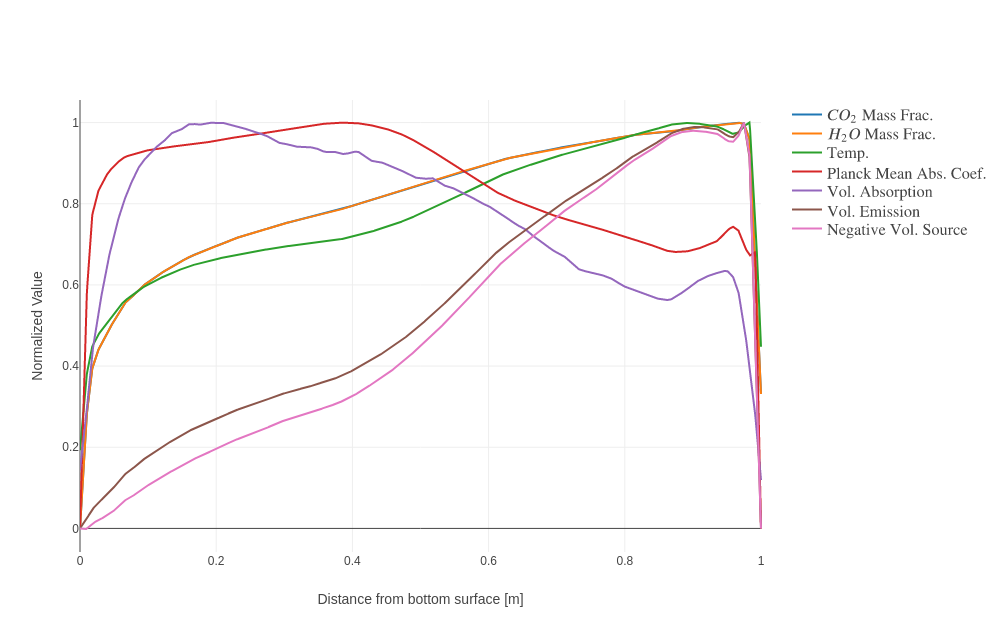
\includegraphics[width=\linewidth]{figures/ch4/line_plot.png}
\caption{Various parameters along the center-line of a gray flame. Values normalized by maximum values along the sampled line.}
\label{fig:PoolFire_lineplot}
\end{figure}


\begin{figure}[!ht]
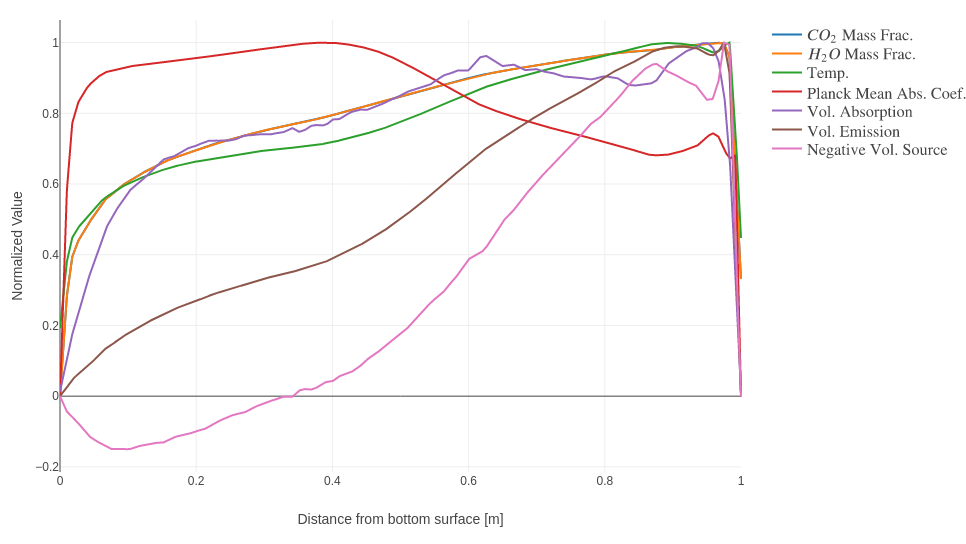
\includegraphics[width=\linewidth]{figures/ch4/line_plot_nongray.png}
\caption{Various parameters along the center-line of a non-gray flame. Values normalized by maximum values along the sampled line.}
\label{fig:PoolFire_lineplot_nongray}
\end{figure}

\subsubsection{Time-accurate simulation}
The same pool-fire is simulated from initial conditions until 4 seconds of physical time.
The simulation is run with line-by-line accurate non-gray emission and radiation source terms are updated each simulation time-step. Chemistry is infinitely-fast, and the case setup is identical to that of the frozen-field analysis.
Several time-steps of the simulation are present in fig. REF. The pool fire is shown to first appear as a mushroom up from the inlet, the reacting, billowing cloud rises upwards, and finally exits through the top boundary of the domain.
The pool fire periodically fluctuates according to a \textit{puffing period}. These oscillations are buoyancy driven and result in 


\subsection{Profiling}
\subsubsection{Single time-step}
The runtimes of various sections of the radiation solver are presented in table \ref{table:RadProfiling} for both CPU and GPU simulations.


\subsubsection{Time-accurate simulation}
Mean and standard deviations of runtimes for the time-accurate simulation are presented in table \ref{table:PoolFireTransient_runtime_table_1rpc}. This simulation is conducted with adaptive emission, totalling approximately 3,400,000 rays emitted and traced per time-step.


\begin{table}[h!]
\centering
\begin{tabular}{||c c c c||} 
 \hline
 Parallel Variation & Radiation Execution & Total Execution & Percent contribution \\ [0.5ex] 
 \hline\hline
 30 CPU processors & 8100s($\pm{}$578s) & 21657s($\pm{}$844.8s) & 37.4\%($\pm{}$2.1\%) \\ 
 GPU & N/A & 6.91 s & - \\
 \hline
\end{tabular}
\caption{Mean runtime contribution of radiation per timestep compared to total runtime. Standard deviations are present in parenthesis. List CPU runtimes consist of radiation parallelized on 30 CPU processors, and CFD calculation occuring on 1 processor. GPU runtimes consist of radiation running on the GPU and CFD calculated using 1 CPU processor.}
\label{table:PoolFireTransient_runtime_table_1rpc}
\end{table}

It should be noted that the runtimes present in table \ref{table:PoolFireTransient_runtime_table_1rpc} include the loading of both the mesh and the line-by-line database for each timestep. Future work will include pre-loading the database once at the beginning of the simulation to reduce the overhead associated with the file I/O.
Following the profiling results present in the previous section, loading of the LBL database requires up to 


\section{Pratt \& Whitney aircraft engine Combustor}
A three dimensional Pratt \& Whitney combustor  \textbf{(Block C)}? geometry was next tested for verification and profiling of the present radiation model. Solver profiling is presented alongside general observations regarding the effects of radiation within the system.
The combustor geometry follows a Rich-Quench-Lean (RQL) configuration, an optimal design for both emissions and stability.
A single time-step from an LES of the combustor was taken for a frozen-field analysis. The effects of soot, spectral emission patterns, and wall-incident radiation were all captured within the model, and detailed account of these effects alongside profiling of the various parallel implementations of the model are presented as demonstration.
The effects of liquid fuel spray on ray-scattering and absorption are neglected.

The combustor geometry is constructed to for highly turbulent flow with a high degree of separation to allow for a sufficiently stabilized flame.
A re-circulation zone immediately behind the inlet section induces a swirl which facilitates mixing of the reactants, and a downstream dilution hole results in a complex chemical mixing process for the remaining reactions to occur in a fuel-lean condition. 



\subsection{Case setup}
The combustor geometry is meshed into a grid of 16,373,876 hexahedral cells of varying shapes and sizes. The simulation is completed with adaptive emission.



\textbf{Unknowns:}
\begin{enumerate}
    \item Was the LES conducted with an alternative radiation model previously?
    \item Were spray droplets included in the study?
\end{enumerate}

Figure ref{} displays normalized temperature profiles throughout the combustor geometry.


\begin{table}[h!]
\centering
\begin{tabular}{||c c c c||} 
 \hline
 Col1 & Col2 & Col2 & Col3 \\ [0.5ex] 
 \hline\hline
 1 & 6 & 87837 & 787 \\ 
 2 & 7 & 78 & 5415 \\
 3 & 545 & 778 & 7507 \\
 4 & 545 & 18744 & 7560 \\
 5 & 88 & 788 & 6344 \\ [1ex] 
 \hline
\end{tabular}
\caption{Runtime comparisons for the Pratt \& Whitney combustor geometry.}
\label{table:PW_runtime_table}
\end{table}
